\documentclass[11pt,
%twocolumns
a4paper, 
swedish, english]{article}
\pdfoutput=1


\usepackage{custom_as}

\graphicspath{ {Figures/} }
\usepackage[margin=10pt, font=small]{caption}
%%För att lägga in 'att göra'-noteringar i texten
\usepackage{todonotes} %\todo{...}, \todolist


%%För att själv bestämma marginalerna. 
\usepackage[
            top    = 3.5cm,
            bottom = 3.5cm,
            left   = 3cm, right  = 3cm
]{geometry}

%%För att ändra hur rubrikerna ska formateras
%\renewcommand\thesection{...}




\begin{document}

\title{A novel method for measuring the acceleration of gravity --
  Encouraging students' experimental creativity} 

\newcommand{\andsunds}{andsunds@chalmers.se}
\author{Andréas Sundström\footnote{Engineering Physics, Chalmers
    University of Technology, Gothenburg, Sweden,
    \textcolor{blue}{\href{mailto:\andsunds}{\nolinkurl{\andsunds}}} }
\and Tom Adawi\footnote{Engineering Education Research, Chalmers
  University of Technology, Gothenburg, Sweden} 
}
\date{\today}

\maketitle

\begin{abstract}
    This article describes an inexpensive yet experimentally
    challenging method for measuring the acceleration of gravity, $g$,
    using a rotating liquid surface and a laser pointer. The main idea
    underpinning this novel method is that a rotating liquid surface
    will form a parabolic reflector which will focus the light to a
    known focal point. By measuring the height of this focal point, $g$
    could be determined to $\unit[9.78 \pm 0.13]{m/s^2}$. We briefly discuss the
    pedagogical merits of this method compared to more traditional
    methods for measuring $g$, and how it can be implemented as an
    experimental problem at different educational levels. 
\end{abstract}





\section{Introduction}

The acceleration of gravity, $g$, has been measured countless times in
secondary school physics laboratories. This is usually done through
some sort of pendulum or free fall experiment. In terms of
experimental simplicity these methods are hard to beat. On the other
hand, these methods do not excite much experimental creativity. In
these cookbook-style labs, the students follow step-by-step
instructions and there is little room for intellectual engagement. As
pointed out in~\cite{Domin1999}, ``Recipe-like activities often short
circuit opportunities to stimulate thinking by
students''. Consequently, cookbook labs have very limited impact on
students' understanding of the nature and practice of
science~\cite{Domin1999}. 

In this paper, we describe a novel and more thought-provoking way to
measure the acceleration of gravity. The idea of the method is to
study the surface of a liquid in a rotating bowl. The surface will
form a parabolic reflector, which will focus incoming planar
light. This is a property of parabolic mirrors most of us are familiar
with, but have never observed directly. By measuring \todo{Beskriv hela
idén/metoden här, inkludera uttrycket för g som används så det blir
tydligare hur mätningen går till och nämn att härledning diskuteras i
sektionen som vi kallar ``theoretical background''}

% A more thought-provoking way to measure $g$ is to study the surface of
% a liquid in a rotating bowl. More precisely, the surface will
% form a parabolic mirror, which will focus incoming planar light. This
% is a property of parabolic mirrors most of us are familiar with, but
% have never observed directly. 

A somewhat similar method has been used as part of an experimental
problem in the International Physics Olympiad,
IPhO~\cite{IPhO2001}. However, in the IPhO problem a 
\todo{kanske kan förtydliga vad det är}
different aspect of the parabolic surface was used
to determine g. Apart from this, we have not been able to find any
previous reports of experiments that use a rotating liquid surface to
determine $g$. 


% A similar method have been used as part of an experimental
% problem in the International Physics Olympiad (IPhO\footnotemark{})
% 2001~\cite{IPhO2001}. So this method already have quite good gounds as
% a challenging lab exercise. However, in IPhO a different aspect of the
% parabolic surface was used to determine $g$. Other than this, no
% previous descriptions on the use of a rotating liquid surface to
% dertermine $g$ have been found.
% \footnotetext{IPhO is an international physics competition for
%   talented high school students from about 80 countries. } 

\subsection{Pedagogical reflections}

The experiment to measure the acceleration of gravity described in
this paper could be carried out as a shorter project for secondary
school students or as a laboratory exercise for first-year
undergraduate physics students. One should note though, that the
experiment takes around 2--4~hours from scratch to finished
measurements, depending on the desired experimental accuracy. If this
experiment is conducted as a project, the students could compare this
method to more traditional methods for measuring the acceleration of
gravity. 

Traditional laboratory instruction has been criticized for the
emphasis it places on following step-by-step instructions, leaving
little room for intellectual engagement~\cite{Domin1999}. In these
cookbook labs, ``virtually no attention is given to the planning of
the investigation or to interpreting the
results''~\cite{Domin1999}. As a consequence, ``virtually no
meaningful learning takes place''~\cite{Domin1999}. As a way to avoid
the cookbook-style lab exercise, the method for measuring the
acceleration of gravity described in this paper could form the basis
for a more open experimental problem. The students could, for example,
be asked to determine the acceleration of gravity using some given
equipment. But as always when there is no ``recipe'' to follow,
unintended solutions might appear – like the one
in~\cite{IPhO2001}. This is, however, not necessarily a bad thing. As
Pickering noted, in cookbook labs, students are never ``orced to
reconcile results, or confronted with challenge to what is naively
predictable''~\cite{Domin1999}. 

The instruction to determine something using a given set of equipment
and with no further information regarding the procedure, is common in
physics competitions, like the IPhO. An experimental problem with this
type of minimal instruction, might therefore be more suited for
students who already have a good understanding of physics. Although
this type of minimal instruction is common in the IPhO, the
experimental problem in 2001~\cite{IPhO2001} included quite a few
hints. This indicates that the concept of measuring the acceleration
of gravity with a rotating liquid surface could be too challenging for
most secondary school students without additional guidance. The hints
provided in the IPhO experimental problem in 2001 could be used as a
source of inspiration for developing laboratory instructions suitable
for students with different levels of background knowledge and at
different educational levels. 



\subsection{Initial theoretical analysis}
To show that a liquid in a rotating vessel will form a parabolic
surface, one can either study the forces on the liquid in the rotating
frame of reference or simply start with some dimensional analysis. The
study of the forces have been done before~\cite{Sabatka2010, Berg1990}
and are not that hard to do. As to not repeat what's already been
done, a short dimesional analysis is presented here instead of the
full derivation. 

All symbols used in the following sections are given in
\figref{fig:rot_bowl}. 

\begin{figure*}\centering
\resizebox{.6\linewidth}{!}{\input{Figures/rot_bowl.pdf_t}}
\caption{Schematic drawing of the setup together with the definitions
  of the notation used in the calculations. Due to the focal height
  being measured slightly outside the exact center of the rod, by
  $\rho$, a small correction $\delta$ has to be made to the measured
  focal height.} 
\label{fig:rot_bowl} 
\end{figure*}

\subsubsection{Dimensional analysis}
The method in this article relies on the fact that the surface is
parabolic, but it won't use this dimensional analysis any further than
as a novel way to, almost, derive the formula of the surface in a
rotating bowl. 

To begin with, an assessment of which parameters will affect $z$ must
be made. One can here convince oneself that $z$, ideally, should be a
function of the three parameters $r$, $\omega$, and~$g$. If a power
law is assumed, the relationship can be written as
\begin{equation}
z\propto r^a\, \omega^b\, g^c.
\end{equation}
Here there are three unknown exponents.

However, it's easier to study the relationships of dinesionless
parameters, so $z/r$ is studied instead. Since this is dimensionless,
the relation to $z/r$ must be with other combinations of parameters
which are also dimensionless. The only posible solution is therefore
\begin{equation}\label{eq:dim}
\frac{z}{r} \propto \left(\frac{r\omega^2}{g}\right)^\alpha, 
\end{equation}
where $\alpha$ now is the only unknown exponent.

Furthermore, the surface should be smooth everywhere. In particular,
the center of rotation can be a problem. The only possibility to get a
smooth surface in the center is if $\nicefrac{\rd{z}}{\rd{r}}=0$ when
$r=0$. This and \eqref{eq:dim} leads to the conclusion that $\alpha>0$.

More than this can not be said about the surface given only a
dimensional analysis. Since it's known that the surface should be
parabolic, it follows that $\alpha=1$. 
Which is probably one of the most likely hypothesis a student would've
made at first glance.  

\subsubsection{Theoretical and experimental confirmation}
The dimensional analysis showed that more information is needed to get
the full picture of the situation. To get this, one can look at the
forces acting on the liquid.

By studying the centrifugal force in the rotating frame of reference
alongside gravity, it can readily be shown that the gradient of the
liquid surface will be proportional to the distance from the axis of
rotation. This corresponds to a parabola. 

More precisely the surface will follow the
equation~\cite{Sabatka2010, Berg1990} 
\begin{equation}\label{eq:parabola}
z(r)=\frac{r^2\omega^2}{2g}.
\end{equation}
In 2010 \v{S}abatka and
Dv\v{o}rák~\cite{Sabatka2010} confirmed this experimentally using a
set of metal rods. 


\subsection{Description of the experiment }
The fact that the surface is parabolic can then be used optically. A
parabolic mirror will reflect any vertically incoming light to the
focal point of that parabola. This property was used by
Berg~\cite{Berg1990} in 1990 to focus light into an optical
image. There's even a telescope, the Large Zenith
Telescope~\cite{LargeZenith}, which uses a rotating mercury mirror. 

The focus of the parabola in \eqref{eq:parabola} is located at the
height~\cite{Physics_Handbook} 
\begin{equation}
h=\frac{g}{2\omega^2}
\end{equation}
above the vertex of the parabola. So by locating the focal point of
the parabola in \eqref{eq:parabola} the value of $g$ can then be
calculated as 
\begin{equation}
g=2h\omega^2.
\end{equation}
As we can see here, only the focal height $h$ and the angular
frequency $\omega$ influence the value of $g$ making this method
experimentally quite clean with only two parameters to measure. 

Neither of these steps require very complicated theoretical calculations, but
the steps are not all trivial. All in all, this method will
give the students an exercise in combining knowledge from two parts
of physics. At the same time the student's experimental creativity can
be used as there are many ways of locating the focal point. 




\section{Method and apparatus}
The apparatus shown in \figref{fig:rot_bowl_pic} consists of a bowl of water
on a spinning disk, a laserpointer, a central rod marking out the axis of
rotation, and a photodiode for measuring the speed of rotation. The spinning
disk was driven by a DC motor so the rotational speed could be
adjusted by varying the voltage applied on the motor. 

The focal point will be located somewhere along the axis of rotation. So when
shining a laser vertically down on the parabolic surface, the refection will hit
the central rod at the height $h$ over the vertex, which can be measured
using a narrow ruler. 

Then by varying the rotational speed and measuring the focal height for
different speeds, a linear regression could be made for $g$ as the
slope of the curve of $h$ plotted against $1/(2\omega^2)$. 
Measurements were taken at two different radial distances from the
center to verify that the radial distance has no impact on the measured
value of $g$. 

The rotational speed $\omega$ was measured with a photodiode connected
to a digital oscilloscope which could record several periods of
rotation. Though a more readily available option, is to connect the
photodiode to a computer's microphone input and record the signal as a
``sound'' file on the computer, as~\cite{Sabatka2010} did. Since
$\omega$ is one of the two parameters directly determining the value
of $g$, it's recommended to measure the periods with some kind of
digital logging device such as an oscilloscope or computer, to
minimize uncertainty in this parameter.

\begin{figure}
\centering
\resizebox{6cm}{!}{\input{Figures/rot_bowl_pic.pdf_t}}
\caption{A photograph of the setup running. The
  reflected beam from a laser pointer (outside frame) can be seen at
  the focal point on the central rod. } 
\label{fig:rot_bowl_pic} 
\end{figure}

\subsection{Calibration}
Firstly the laser pointer has to be perfectly vertical. This can neatly be
calibrated by shining the laser down on the water surface when it's not
rotating. The laserbeam will be perfectly vertical when the
reflection hits the source, due to the water surface being perfectly
horizontal when still.

To get the central rod centered, a center mark was put in the rotating
disc. A spirit level was used to ensure that the central rod was
vertical. Both of these steps are essential, since deviation from the
center will change the measure value of $g$, as we will see in next
section. 


\subsection{Correction}\label{sec:corrections}
As shown in \figref{fig:rot_bowl} the measured focal height
$\hat{h}$ is slightly off from the real focal height by 
\begin{equation}%\label{eq:correction}
\delta=\rho\cot 2\alpha
\end{equation}
due to a finite width, $\rho$, of the central rod. This width is easily
measured with a pair of calipers.

We now have to determine $\alpha$. First of we note that
\begin{equation}\label{eq:dz/dr}
\tan\alpha=\dv{z}{r} =\frac{2 z(r)}{r}.
\end{equation}
Then we see from \figref{fig:rot_bowl} that 
\begin{equation}
\cot 2\alpha =\frac{\hat{h} - z(r)}{\hat{r}} 
= \frac{\hat{h}-\frac{r}{2}\tan\alpha }{\hat{r}},
\end{equation}
where we used \eqref{eq:dz/dr} to substitute $z(r)$ in terms of
$\tan\alpha$. By rewriting the last equation, we get
\begin{equation}
\cot 2\alpha 
-\frac{\hat{h}}{\hat{r}}
+\frac{\hat{r}+\rho}{2\hat{r}}\tan\alpha  = 0.
\end{equation}
only consisting of known or measured quantities and $\alpha$. From
this stage $\alpha$ can easily be obtained to a satisfying degree with
regular numerical equation solvers.



\section{Results}
The results from the measurements together with the least square fitt
are shown in \figref{fig:data}. The calculated value of the
acceleration of gravity comes out as
\begin{equation}
g=\unit[9.78\pm 0.13]{m/s^2}
\end{equation}
the uncertainty given is the standard error in the mean.


\begin{figure*}\centering 
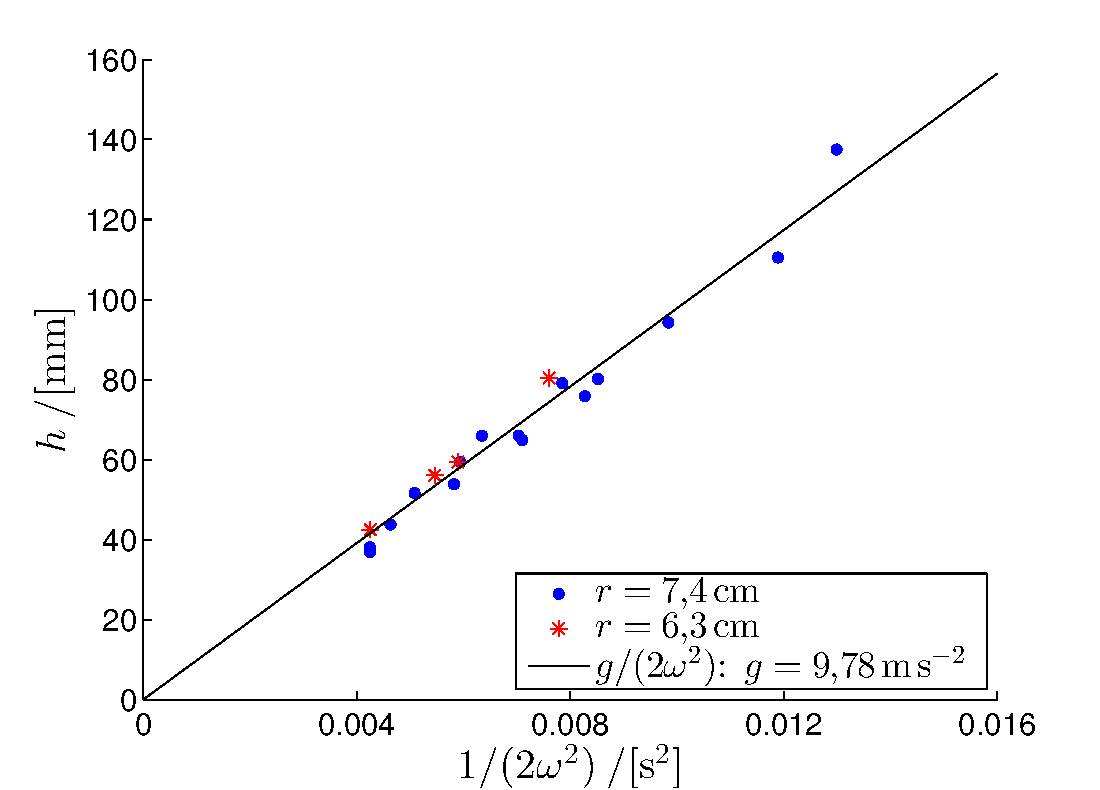
\includegraphics[width=.8\linewidth]{g_minsta_kvadrat.pdf}
\caption{\label{fig:data} Measurements of the focal height $h$ (with
  corrections for a center rod of non-zero width) plotted against
  $1/(2\omega^2)$. The acceleration of gravity $g$ is now given as the
  slope of the least square fitt to these data points. Measurements
  were taken at two different radial distances from the center,
  denoted $r$ in \figref{fig:rot_bowl}.
}
\end{figure*}



\section{Discussion}
Since this is a completely new method of measuring $g$, it is not
easy to compare this particular result to other's. The closest
comparison we can make is to the results in
IPhO~2001~\cite{IPhO2001}. In the solutions to their problem
they state that $g$ could be measured to
$\unit[9.8]{m/s^2}$ with a standard error of $\unit[0.2]{m/s^2}$. So
compared to these results, ours seems to be at least as good, or perhaps
even a little better than other methods using a rotating liquid. 

With this said, the error in this method is considerably larger than
some of the most sophisticated pendulum methods~\cite{Candela2001}. But
as stated before, this method is more of an educational experiment
than a precision measurement. And as such, this experiment manages to
combine both knowledge in mechanics and optics, together with some
careful thought needed, for example to find the correction $\delta$. 

The significance of the correction due to finite width of the central
rod, $\delta$, is quite notable. The value of $g$ comes out to be only
about $\unit[9.2]{m/s^2}$ \emph{without} these corrections. This
demonstrates the necessity of the calculations made in
section~\ref{sec:corrections}. 


\subsection{Experimental improvements}
Most of the uncertainty in the result arose from small ripples on the
water surface leading to a jittery motion of the reflected
laser beam. Both Berg~\cite{Berg1990} and IPhO~\cite{IPhO2001} used
glycerin as the liquid in their experiments. Due to the high viscosity
of glycerin, the ripples causing the uncertainties would have lessened.
However, as this experiment was primarily aimed as an experiment with a
simple and inexpensive setup we used water instead.  

Another way to increase accuracy would be to use a bigger bowl,
preferably a bowl with vertical walls. Because the maximal rotational
speed will be limited by the slope of the walls, since the walls have
to have a steeper slope than the water surface.

There's also other way to locate the focal point. For example, two
different laser could be used. By shining the two laser beams
vertically down at two different points on the rotating surface, the
focus is then located at the point of intersection od the reflected
beams. This will eliminate the need to calculate the correction in
section~\ref{sec:corrections}. 

\subsection{Pedagogical merits}
The experiment described here can be done as a shorter project in high
school or lab exercise for first year undergraduate students. One
should note though, that to set up this experiment will take around
2--4~hours from scratch to finished measurements, depending on the
desired experimental accuracy. If this experiment is done as a
project, the student could perhaps also try to compare this method to
other more common methods.

As a way to move away from expository lab exercises, the method in
this article could be given as a more open problem to the
students. Depending on to what degree of replication of this method
is wanted, the student could for example be asked to determine $g$
using only some given equipment. But as always when there's no
``recipe'' to follow, some unintended solutions might appear --- like
the one in \cite{IPhO2001}. Although this might not be an entirely bad
thing. 

The instruction, to determine something using a given set of
equipment and no information regarding the procedure, is very similar
to how a contestant in physics competitions, like IPhO, is presented
with their problems. Therefore an exercise set up with these minimal
instructions, might be most suited for students who already have a
good understandig of physics. 

Although these minimal instructions are common in IPhO, the problem in
2001~\cite{IPhO2001} had quite a lot of hints given to the
contestants. This indicates that the concept, of measuring $g$ with a
rotating liquid surface, could be too challenging for most students
with out help. Perhaps one could base a laboratory instruction in the
problem instructions given in \cite{IPhO2001}. 



\section{Conclusion}
This is a new, quite out of the ordinary, method to measure the
acceleration of gravity $g$. As an experimental method, it fares well
compared to similar methods~\cite{IPhO2001}, but not as well to some
of the most accurate methods~\cite{Candela2001}. 

As a laboratory exercie, this method might prove quite challenging to
most students. But with sufficient help, the student will have used a
wide variety of different knowelge to reach the end result. The
student will also have seen the focusing property of parabolic mirrors
demonstrated while doing this experiment.




\section*{Acknowledgments}
We are very grateful to the personell in the machineshop at the
Physics Department at Chalmers. We thank Lars Hellberg and Jan-Åke
Wiman for constructing and balancing the rotating disk so that the
experiments could be performed. 



%Bibliography
\bibliographystyle{ieeetr}
\bibliography{bibliography}

\end{document}